\chapter{Building the Foundation — Data and First Prototype}\label{chapter:BF-DFP}


\section*{Introduction}
\addcontentsline{toc}{section}{Introduction}
After studying how SmartCare works and going through its documentation, one thing was immediately obvious --- this isn't a platform you can just plug into and start pulling data from. 
SmartCare is a commercial solution deployed by Huawei across many of its
customers worldwide, so any data it contains is confidential by nature, and
attempting to access or alter it directly would affect the privacy of live
operator environments. 

So it isn't an option to just pull data from there. To
ensure confidentiality while still building something realistic, we turned to
the TM Forum framework --- the open industry standard that defines the data
models and component architecture used across the telecom industry. SmartCare
itself is a TM Forum ODA-certified product \cite{huawei_tmforum}, meaning its
structure follows the same standard as any other ODA-certified product.

Using TM Forum's component taxonomy \cite{tmforum_sid} as our reference, we designed
a database that replicates most of the necessary data a platform like SmartCare
would operate on, without relying on any confidential information. From there,
we built two SQLite databases populated with \(\sim\)50{,}000 synthetic
subscribers. This is what the agent works on throughout the rest of the project.
\section{Database Design}\label{sec:db-design}

The data layer is split into two separate SQLite databases, each with a distinct
 responsibility --- a separation that mirrors the classic OSS/BSS divide in telecom 
 architecture \cite{tmforum_sid}.

The two databases are linked by a single key --- the \texttt{msisdn}, which is 
the subscriber's phone number. Every table on both sides that relates to a specific
subscriber uses the \texttt{msisdn} as its identifier, making cross-database joins
straightforward. 

This design keeps network and commercial data cleanly separated
while still allowing the agent to query across both when needed --- for example,
correlating a subscriber's poor QoE scores with their churn risk and current
plan.
This design was chosen in order to keep network and commercial data seperated
while still allowing the agent to query across both, giving us cleanliness as 
well as we get to test the agent's ability to make cross DB queries. 
The schema was designed to cover the main data domains that TM Forum's Information Framework defines for a telecom operator \cite{tmforum_sid}: resource and network management, service usage, customer and party management, billing, and product catalog.

\subsection{Network Database}

\texttt{NetworkAnalyzer\_new.db} covers everything on the network and
operational side, organized into six groups (Table~\ref{tab:schema-network}).

\begin{longtable}{@{}p{2.1cm}p{3.5cm}p{8.2cm}@{}}
\caption{\texttt{NetworkAnalyzer\_new.db} --- the network and operational
side.}\label{tab:schema-network}\\
\toprule
\textbf{Group} & \textbf{Table} & \textbf{What it holds} \\
\midrule
\endfirsthead
\toprule
\textbf{Group} & \textbf{Table} & \textbf{What it holds} \\
\midrule
\endhead
Infrastructure & \texttt{sites} & Base station locations across 21 regions and 24 cities \\
 & \texttt{cells} & Radio cells per site, with technology (2G--5G) and frequency band \\
\addlinespace
Subscribers & \texttt{subscribers} & Core identity and location \\
 & \texttt{subscriber\_technology} & Active technology and VoLTE status \\
 & \texttt{devices} & Handset capability: 5G, VoLTE, Wi-Fi calling \\
 & \texttt{coverage} & Which cells a subscriber can reach from home \\
\addlinespace
KPIs & \texttt{kpis\_daily} & Per-cell daily RSRP, SINR, throughput, drop rate, latency, congestion \\
 & \texttt{kpis\_hourly} & The same at hourly grain, for intraday analysis \\
\addlinespace
Usage & \texttt{dou\_monthly} & Total data used per subscriber per month \\
 & \texttt{ott\_monthly} & The same split by app category, plus SMS and voice minutes \\
 & \texttt{mobility\_profile} & Distinct cells visited, mobility class, FWA candidacy \\
 & \texttt{roaming\_usage} & Data and voice consumed abroad \\
\addlinespace
Quality of Experience & \texttt{qoe\_daily} & Daily experience score per subscriber per app type \\
 & \texttt{signal\_quality} & RSRP and SINR at subscriber level \\
 & \texttt{streaming\_quality} & Monthly streaming score \\
 & \texttt{web\_quality} & Monthly web score \\
 & \texttt{voip\_quality} & Monthly VoIP score --- only for 4G with VoLTE, or 5G \\
\addlinespace
Operations & \texttt{network\_alarms} & Cell-level faults \\
 & \texttt{network\_incidents} & Cell-level outages \\
 & \texttt{experience\_incidents} & Subscriber-facing incidents, with root cause and timestamps \\
 & \texttt{complaints} & Subscriber-reported issues, categorised by technology tier \\
 & \texttt{nps\_scores} & Monthly Net Promoter Score submissions \\
\bottomrule
\end{longtable}

\texttt{coverage} records reachability from a subscriber's home location rather
than live attachment --- a distinction the agent depends on whenever it counts
who can actually be served by a given cell.

\subsection{Operator Database}

\texttt{operator\_new.db} covers the commercial side, organized into three
groups (Table~\ref{tab:schema-operator}).

\begin{longtable}{@{}p{2.1cm}p{3.5cm}p{8.2cm}@{}}
\caption{\texttt{operator\_new.db} --- the commercial
side.}\label{tab:schema-operator}\\
\toprule
\textbf{Group} & \textbf{Table} & \textbf{What it holds} \\
\midrule
\endfirsthead
\toprule
\textbf{Group} & \textbf{Table} & \textbf{What it holds} \\
\midrule
\endhead
Customers & \texttt{customers} & Profile, demographics, region, segment \\
 & \texttt{subscriptions} & Which plan each subscriber is on, and contract type \\
 & \texttt{plans} & Data caps, speeds, pricing, and 5G/VoLTE/FWA/MBB flags \\
\addlinespace
Financials & \texttt{billing} & Monthly invoices, split into data and voice charges \\
 & \texttt{customer\_value} & ARPU, value segment, churn risk score and label \\
\addlinespace
Campaigns & \texttt{campaigns} & Operator-initiated outreach campaigns \\
 & \texttt{campaign\_targets} & Who each campaign targets, and conversion \\
 & \texttt{offers} & The commercial offers attached to campaigns \\
 & \texttt{offer\_assignments} & Which offer went to whom, and whether it was accepted \\
 & \texttt{sms\_log} & Every notification sent \\
 & \texttt{service\_interruptions} & Outages a subscriber actually experienced \\
 & \texttt{agent\_actions} & Proposals from the agent awaiting human review \\
\bottomrule
\end{longtable}

Churn risk score and label live in \texttt{customer\_value}; how they are
computed, and why the approach changed, is covered in Chapter~\ref{ch:eval}.

\subsection{Schema Overview}

Figure~\ref{fig:schema-overview}, on page~\pageref{fig:schema-overview},
lays out both databases side by side, grouped the same way they were
just described above: the network-side groups (Infrastructure,
Subscribers, KPIs, Usage, Quality of Experience, Operations) on the
left, and the commercial-side groups (Customers, Financials, Campaigns)
on the right. The single connector between them is
\texttt{msisdn} — every subscriber-linked table on either side carries it,
which is what makes a cross-database question (``correlate this
subscriber's QoE with their churn risk and current plan'') a plain join.

The grouping here is not just illustrative either
--- it is close to literally how the agent's own schema retriever
organizes itself: every table gets tagged with its owning database, and
that tag is what routes a question before a single query gets written.

\begin{figure}[H]
\centering
\definecolor{netblue}{HTML}{4A6FA5}
\definecolor{opbrown}{HTML}{B5793A}
\resizebox{\textwidth}{!}{%
\begin{tikzpicture}[
  netgroup/.style={rectangle, rounded corners=3pt, draw=netblue, thick,
    fill=netblue!6, align=left, text width=5.4cm, inner sep=7pt, font=\footnotesize},
  opgroup/.style={rectangle, rounded corners=3pt, draw=opbrown, thick,
    fill=opbrown!8, align=left, text width=5.4cm, inner sep=7pt, font=\footnotesize},
]

% ---- left column: NetworkAnalyzer_new.db ----
\node[netgroup, name=g1] {\textbf{\normalsize Infrastructure}\\[3pt]
  $\bullet$~\texttt{sites}\\ $\bullet$~\texttt{cells}};
\node[netgroup, name=g2, below=5mm of g1] {\textbf{\normalsize Subscribers}\\[3pt]
  $\bullet$~\texttt{subscribers}\\ $\bullet$~\texttt{subscriber\_technology}\\
  $\bullet$~\texttt{devices}\\ $\bullet$~\texttt{coverage}};
\node[netgroup, name=g3, below=5mm of g2] {\textbf{\normalsize KPIs}\\[3pt]
  $\bullet$~\texttt{kpis\_daily}\\ $\bullet$~\texttt{kpis\_hourly}};
\node[netgroup, name=g4, below=5mm of g3] {\textbf{\normalsize Usage}\\[3pt]
  $\bullet$~\texttt{dou\_monthly}\\ $\bullet$~\texttt{ott\_monthly}\\
  $\bullet$~\texttt{mobility\_profile}\\ $\bullet$~\texttt{roaming\_usage}};
\node[netgroup, name=g5, below=5mm of g4] {\textbf{\normalsize Quality of Experience}\\[3pt]
  $\bullet$~\texttt{qoe\_daily}\\ $\bullet$~\texttt{signal\_quality}\\
  $\bullet$~\texttt{streaming\_quality}\\ $\bullet$~\texttt{web\_quality}\\
  $\bullet$~\texttt{voip\_quality}};
\node[netgroup, name=g6, below=5mm of g5] {\textbf{\normalsize Operations}\\[3pt]
  $\bullet$~\texttt{network\_alarms}\\ $\bullet$~\texttt{network\_incidents}\\
  $\bullet$~\texttt{complaints}\\ $\bullet$~\texttt{nps\_scores}};

\node[draw=netblue, thick, rounded corners=6pt, fit=(g1)(g2)(g3)(g4)(g5)(g6),
  inner sep=10pt,
  label={[font=\bfseries, label distance=8pt]above:NetworkAnalyzer\_new.db\ (network domain)}]
  (leftbox) {};

% ---- right column: operator_new.db — Financials anchored to leftbox's ----
% ---- vertical middle, Customers/Campaigns built up/down from there ----
\node[opgroup, name=h2] at ($(leftbox.east)+(4.5cm,0)$)
  {\textbf{\normalsize Financials}\\[3pt]
  $\bullet$~\texttt{billing}\\ $\bullet$~\texttt{customer\_value}};
\node[opgroup, name=h1, above=8mm of h2] {\textbf{\normalsize Customers}\\[3pt]
  $\bullet$~\texttt{customers}\\ $\bullet$~\texttt{subscriptions}\\ $\bullet$~\texttt{plans}};
\node[opgroup, name=h3, below=8mm of h2] {\textbf{\normalsize Campaigns}\\[3pt]
  $\bullet$~\texttt{campaigns}\\ $\bullet$~\texttt{campaign\_targets}\\
  $\bullet$~\texttt{offers}\\ $\bullet$~\texttt{offer\_assignments}\\
  $\bullet$~\texttt{sms\_log}\\ $\bullet$~\texttt{service\_interruptions}};

\node[draw=opbrown, thick, rounded corners=6pt, fit=(h1)(h2)(h3),
  inner sep=10pt,
  label={[font=\bfseries, label distance=8pt]above:operator\_new.db\ (commercial domain)}]
  (rightbox) {};

% ---- msisdn connector ----
\draw[<->, thick] (leftbox.east) -- (rightbox.west);
\node[fill=yellow!15, draw, rounded corners, align=center, font=\ttfamily\bfseries,
  inner sep=5pt] at ($(leftbox.east)!0.5!(rightbox.west)$)
  {msisdn\\ {\normalfont\itshape\footnotesize shared join key}};

\end{tikzpicture}%
}
\caption{Schema overview: table groupings in each database, joined on \texttt{msisdn}.}
\label{fig:schema-overview}
\end{figure}

\subsection{Design Rationale}

A few choices behind the schema are worth calling out, since they shaped
everything built on top of it later. First, SQLite doesn't require a server
to stand up, perfect for this project, just a single portable file per
database,  and more than enough for roughly \textasciitilde50{,}000
First, SQLite: no server to stand up,
a single portable file per database, and more than enough for \textasciitilde50{,}000
subscribers — for a prototype at this scale, anything heavier would have
been overkill.

Second, the two-database split. It would have been simpler, technically,
to dump everything into one file. But keeping network and commercial data
apart mirrors the real OSS/BSS boundary operators actually work with, and
it turned out to matter later: the agent needs to decide which domain a
question belongs to before it can write a query, and having that boundary
already baked into the data made that routing logic far more natural than
if everything lived in one undifferentiated pile of tables.

Third, the join key. Every subscriber-linked table on both sides uses a
single \texttt{msisdn} column, with no foreign key constraints enforced.
SQLite barely enforces them anyway, so nothing was really lost. The
trade-off is deliberate: referential integrity becomes the generation
code's job instead of the database's. Fine trade, since every row in
this environment is written by scripts we control in the first place.


\subsection{Confidentiality Through a Fictional Geography}\label{sec:fictional-geography}

Even though the schema itself is grounded in TM Forum's real abstractions,
none of the region, city, or site names in the data are real --- they are
entirely invented. This was a deliberate choice, and it is worth being precise
about why, because a reader encountering unfamiliar place names in an
engineering report is entitled to ask whether they are a joke.

Giving synthetic regions recognizable real-world names would create an
association with an actual country or an actual Huawei customer network that
simply is not there, and that is exactly the kind of confusion this project
needed to avoid from day one. A file of invented subscribers living in real
cities invites exactly the wrong question --- \emph{is this data from that
operator?} --- and the answer being no is not much protection once a screenshot
leaves the room.

The alternative, naming regions \texttt{Region A} through \texttt{Region U},
was considered and rejected for a specific reason: it is not memorable enough to
be checked. Over a project this size the same regions are queried, charted and
argued about hundreds of times, and distinguishable names make an inconsistency
visible where indexed labels hide it. A subscriber in the wrong region is
obvious when the regions have identities; it is invisible when they are letters.

So every region, city, and site name in the data comes from one consistent
invented world, which gives the environment a coherent identity while being
unmistakable for any real operator's network. The names are arbitrary with
respect to the engineering: nothing in the schema, the queries, or the results
depends on them, and substituting a different naming scheme would change no
result in this report. Figure~\ref{fig:ch2-fictional-data} shows what the
invented geography looks like at scale.

% =====================================================================
% SCREENSHOT NEEDED --- figures/ch2-fictional-data.png
% Where: any SQLite browser (DB Browser for SQLite) open on
% NetworkAnalyzer_new.db, OR the analytics dashboard's Subscribers
% section (localhost:8002).
% What to capture: a handful of rows from the subscribers table (or the
% dashboard's subscriber list) with the region/city columns visible,
% clearly showing the invented place names rather than real ones.
% =====================================================================
\begin{figure}[H]
\centering
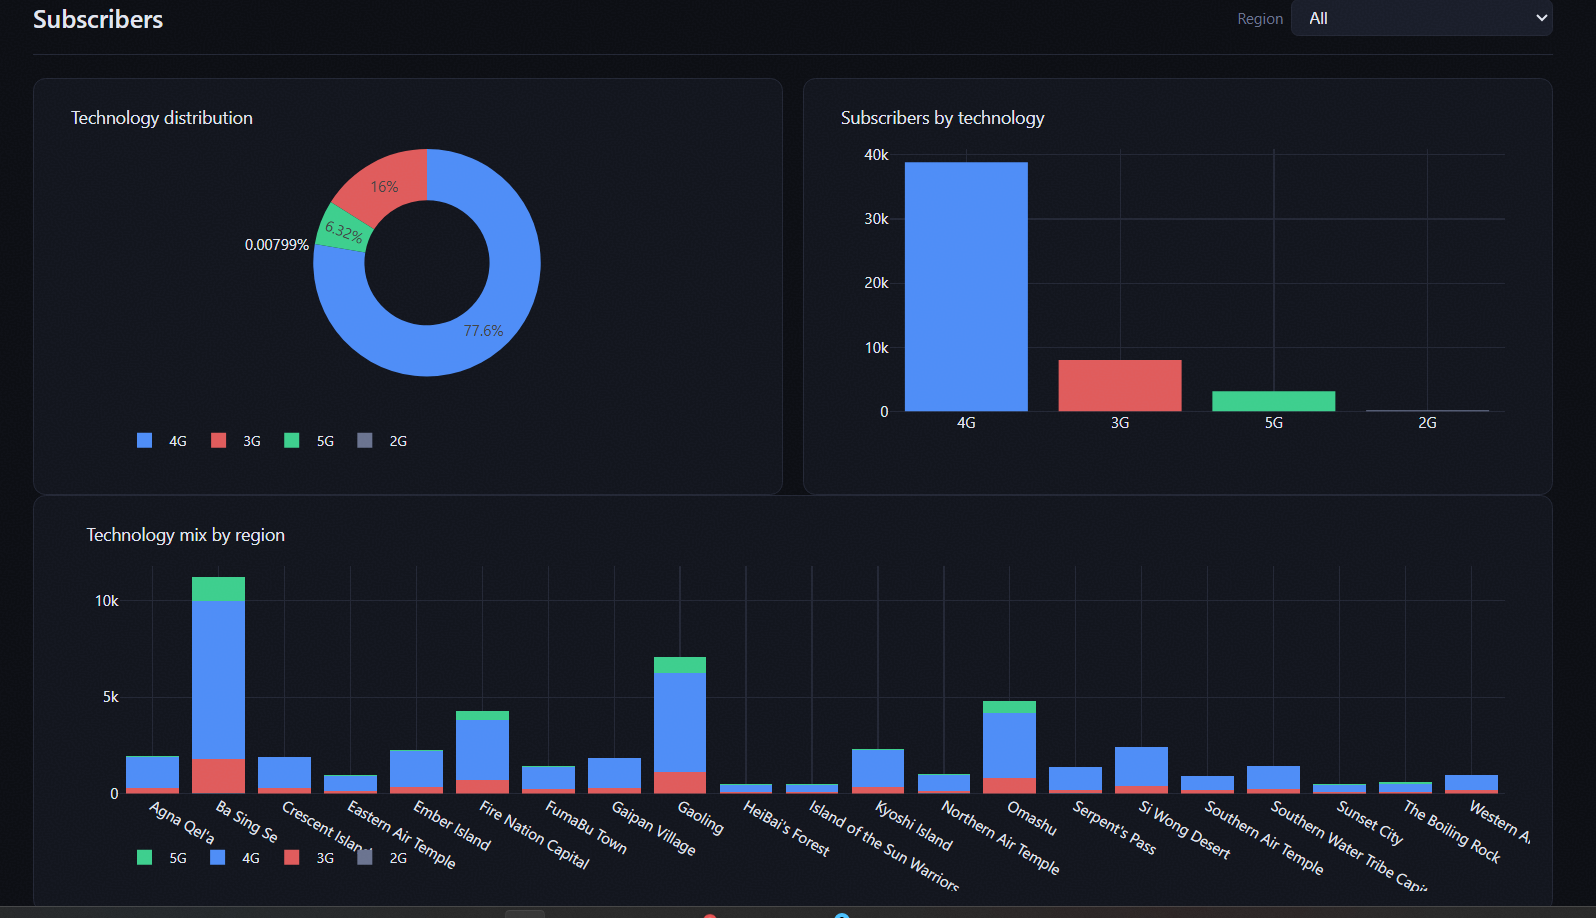
\includegraphics[width=0.85\textwidth]{figures/ch2-fictional-data.png}
\caption{Subscriber technology mix by region, from the live database. The region
names are fictional; the data behind them is internally consistent.}
\label{fig:ch2-fictional-data}
\end{figure}

\section{First Prototype: A Local Agent Loop}

With the databases in place, the next question was whether the actual
idea — ask a question in plain English, get a SQL-backed answer — could
work at all before worrying about making it fast or polished. The fastest
way to find out was to wire up a minimal agent loop against a model
running entirely locally, no cloud dependency, no API cost, nothing to
wait on.
\subsection{Getting a Loop Working}
The first version ran on Ollama~\cite{ollama} with a local qwen
model~\cite{qwen} — 7B, later bumped to 8B — driving a single-step
reasoning loop built around plain text tags rather than anything
structured: \ldots the model would read the question and respond with a \texttt{QUERY\_SC:} or \texttt{QUERY\_OP:}
tag followed by raw SQL, the loop would run that query against the
matching database, feed the result back, and repeat until the model
wrote a \texttt{CONCLUDE:} tag with its final answer. No tool-calling
API, no structured output — just a prompt format the model had to follow
by convention, parsed back out with regular expressions on this end.
For the first prototype we used a heavily customized Streamlit app
(Figure~\ref{fig:streamlit-prototype}) --- dark theme, custom fonts, a chat
panel next to a live snapshot area for charts. Streamlit handles layout and
reactivity on its own, so the time went into the agent loop rather than into
frontend code.

Simple and crude as it was, it did prove the core idea worked: the model could
turn a natural-language question into a query against the schema from
Section~\ref{sec:db-design}, chain a couple of query steps together when one
wasn't enough, and land on something coherent. That gave us a green light to
keep going down this path. The tag-based format itself stuck around much longer
than the local models did, and still shows up later in the report as the
fallback path once tool-calling was introduced.

But the very same screenshot also shows the limitations: the question asked for
a drilldown tree of technologies used against terminal capability, and the agent
answered with a dense block of raw counts --- while the ``Live Snapshot'' panel
next to it stayed completely empty. The reasoning loop could get the numbers
right, but numbers like these need to be visually accessible; a chart or a
drilldown tree would do a lot better. So that became another thing to fix.


\begin{figure}[H]
    \centering
    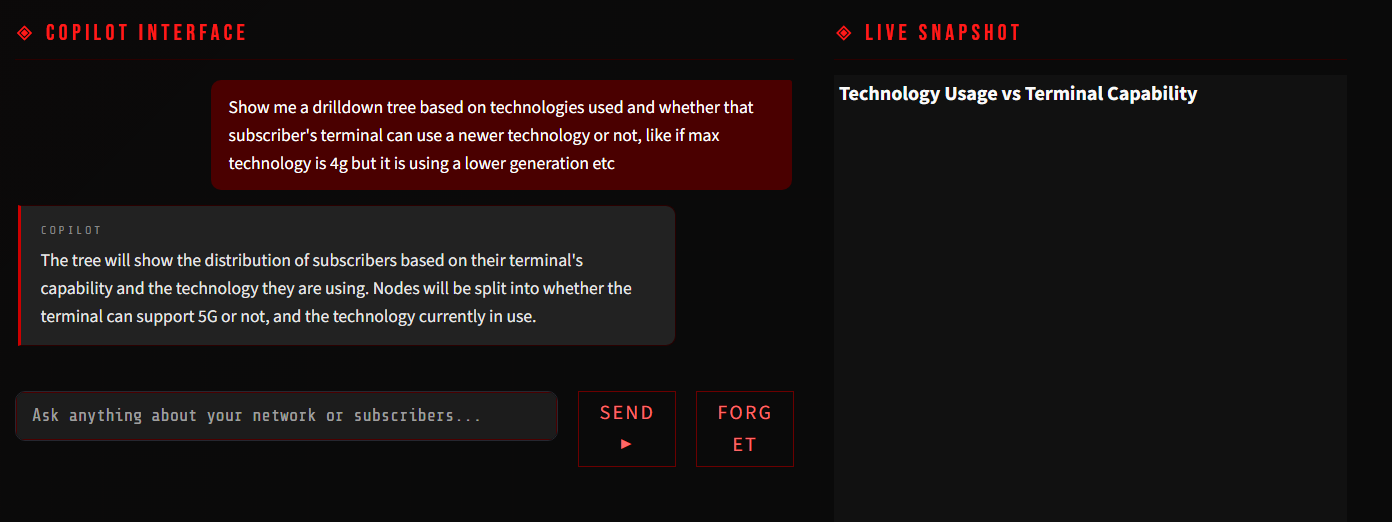
\includegraphics[width=0.9\textwidth]{figures/streamlit_prototype.png}
    \caption{The first Streamlit prototype: a drilldown-tree question answered
    with raw counts and no chart.}
    \label{fig:streamlit-prototype}
\end{figure}


\subsection{Hitting the Hardware Ceiling}

What that first loop did not prove was that local inference was viable to
actually use. It ran on an RTX 3050 with 4~GB of VRAM — enough to load a
7B–8B model, but not enough headroom to serve it at a usable latency once
the prompt included schema context and a few turns of conversation.

Every step of the loop meant another full model call, and with local inference
this slow, a question that should feel instant took far too long. The whole
point of the project was to ask a question and get a thorough answer, and
waiting minutes for one didn't make sense. The impasse was hardware, so we
started looking for alternatives.

\section{The Case for Cloud Inference}

One thing worked in favor of moving the reasoning off-device. Since the
environment was entirely synthetic from the start
(Section~\ref{sec:fictional-geography}), the usual objection to sending
data to a cloud-hosted model simply did not apply — there was no real
subscriber data to protect. That removed the main reason to keep
insisting on local inference, and made the switch a pragmatic step rather
than a fraught one.

Somewhere in the middle of babysitting local qwen3:8b through yet another
sluggish response — close to five minutes for a single prompt to come
back — the whole thing stopped feeling like an engineering trade-off and
started feeling like a bad idea. Both GPU and CPU were pinned the entire
time, since the model did not fit cleanly into 4~GB of VRAM and spilled
over onto the CPU, which raised a more immediate concern than ``is this
the right architecture'': at this rate, was this actually going to fry
the machine?

That is the point this got discussed with a colleague, who, on hearing
``five minutes per prompt,'' asked the obvious question: why not just use
something cloud-hosted instead?

Before that conversation, a local-but-not-quite-local option was briefly
on the table — spinning up a VM through Azure's student credit pack. However that idea
died quickly as the free-tier images do not come with a free GPU or VRAM attached, 
but maybe that was a blessing in disguise as eventually we came across a much more 
efficient solution.
My colleague then suggested using  AWS Bedrock~\cite{aws_bedrock}, which is Amazon's managed
access layer for foundation models. Getting access to \$100 of credit was actually pretty 
simple, I just needed a legitimate card entered, and from there, I got access to lots of 
models, which would normally require a lot of computational force, like qwen3 32B or 80B.
Answers were quick, more precise, and no hardware to worry about.


% =====================================================================
% SCREENSHOT NEEDED --- figures/ch3-bedrock-console.png
% Where: AWS Console -> Bedrock -> Model access (or the Bedrock
% playground/usage page).
% What to capture: the list of enabled foundation models (qwen3-32b /
% qwen3-next-80b-a3b should be visible as "Access granted"), ideally
% with the free usage credit balance visible somewhere on the page too.
% =====================================================================
\begin{figure}[htbp]
\centering
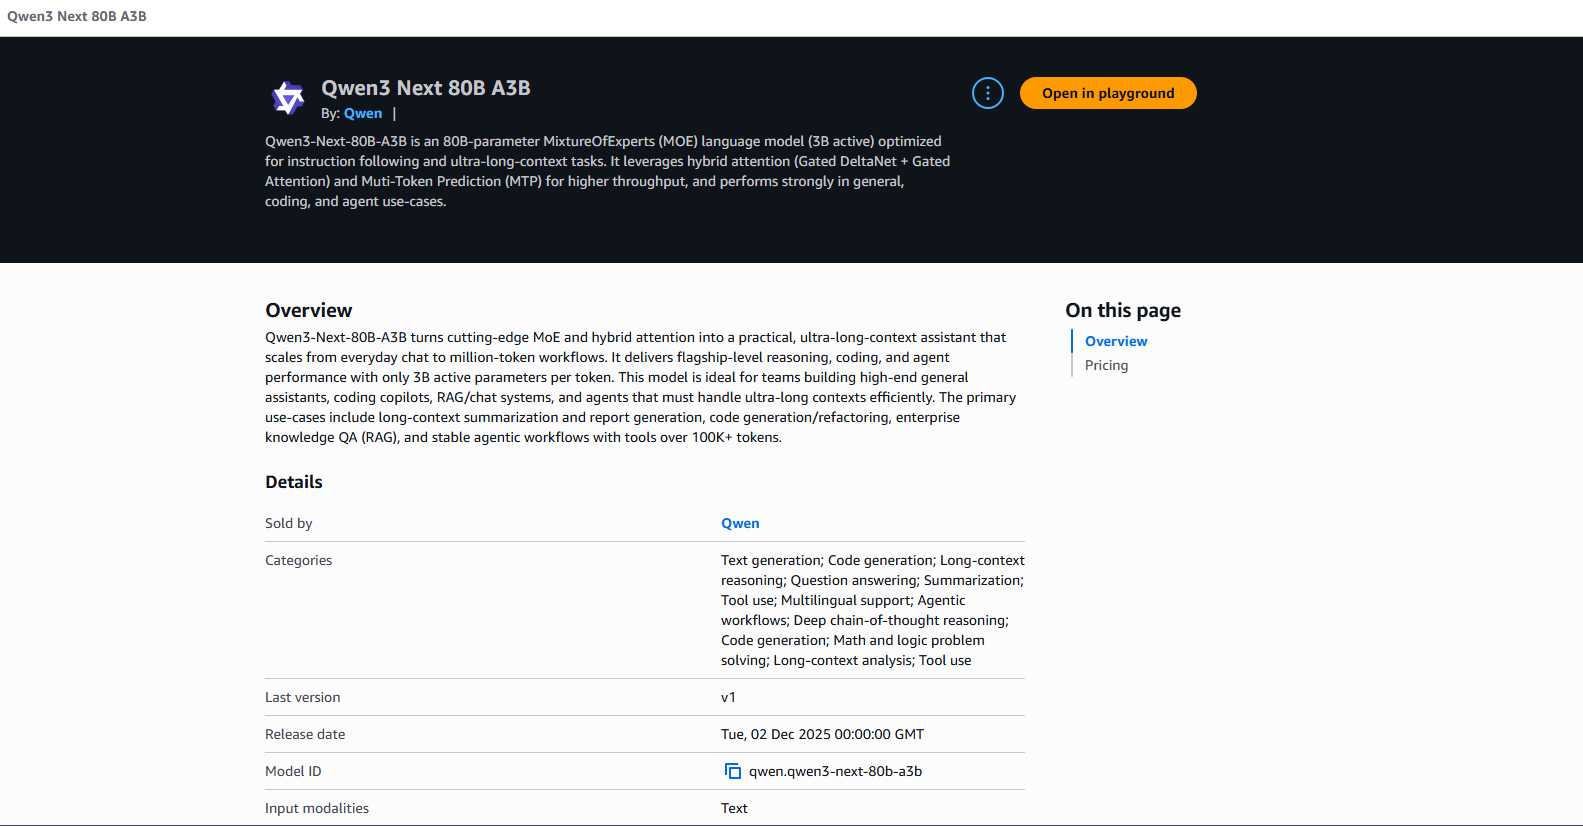
\includegraphics[width=0.85\textwidth]{figures/ch3-bedrock-console.png}
\caption{The AWS Bedrock console showing model access enabled for the
models used in this project.}
\label{fig:ch3-bedrock-console}
\end{figure}

\section{Cleaning Out the Local Stack}

Once cloud inference was clearly the model going forward, the local-model
code that had made up the entire agent up to this point turned into dead
weight rather than a fallback worth keeping around. After that, no more ollama startups, 
launching the server became faster and easier. The old code wasn't outright deleted but
rather archived for the record. 

\section{Making the Cloud Call Reliable}

A local model either answers or it crashes. A network call to a shared
API fails in a completely different way: throttling, timeouts, or the
odd server-side hiccup that has nothing to do with the question being
asked and everything to do with system load at that exact moment.
Treating every one of those as a hard failure would have made the agent
flaky in exactly the way switching to Bedrock was supposed to fix. So
the Bedrock call got wrapped in a retry layer instead: on a transient
error it backs off exponentially and tries again, up to four attempts,
and only retries when nothing had already streamed back so a partial
response never gets duplicated. Small piece of plumbing, but it is the
difference between the agent occasionally failing for no visible reason
and quietly recovering from the kind of hiccup any cloud API throws
from time to time.

% =====================================================================
% System architecture: processes, stores, and what talks to what.
% =====================================================================
\begin{figure}[H]
\centering
\definecolor{procblue}{HTML}{4A6FA5}
\definecolor{storebrown}{HTML}{B5793A}
\definecolor{extgreen}{HTML}{2E8B57}
\definecolor{busamber}{HTML}{C08A2E}
\resizebox{0.95\textwidth}{!}{%
\begin{tikzpicture}[
  proc/.style={rectangle, rounded corners=4pt, draw=procblue, very thick,
    fill=procblue!10, align=center, text width=3.4cm, inner sep=7pt,
    font=\bfseries\footnotesize},
  store/.style={cylinder, shape border rotate=90, aspect=0.22,
    draw=storebrown, very thick, fill=storebrown!12, align=center,
    text width=2.5cm, inner sep=5pt, font=\scriptsize},
  ext/.style={rectangle, rounded corners=4pt, draw=extgreen, very thick,
    fill=extgreen!10, align=center, text width=3.0cm, inner sep=7pt,
    font=\bfseries\footnotesize},
  bus/.style={rectangle, rounded corners=3pt, draw=busamber, very thick,
    fill=busamber!15, align=center, text width=4.0cm, inner sep=6pt,
    font=\scriptsize\ttfamily},
  user/.style={rectangle, rounded corners=3pt, draw=black!55, thick,
    fill=black!5, align=center, text width=2.9cm, inner sep=6pt,
    font=\footnotesize},
  lbl/.style={font=\scriptsize\itshape, align=center, inner sep=2pt},
  flow/.style={-{Latex[length=2.4mm]}, thick},
  biflow/.style={{Latex[length=2.4mm]}-{Latex[length=2.4mm]}, thick},
]

% ---- nodes, placed on explicit coordinates ----
\node[user]  (browser) at ( 0,   0)    {Operator\\[1pt]\normalfont\scriptsize web browser};
\node[proc]  (chat)    at ( 0,  -2.0)  {Chat Server\\[2pt]\normalfont\scriptsize server.py : 8000};
\node[ext]   (bedrock) at ( 6.4,-2.0)  {AWS Bedrock\\[2pt]\normalfont\scriptsize qwen3-32b / 80b-a3b};
\node[proc]  (agent)   at ( 0,  -4.2)  {Reasoning Agent\\[2pt]\normalfont\scriptsize tool loop, grounding,\\verification};

\node[proc]  (sim)     at (-6.9,-7.0)  {Simulator\\[2pt]\normalfont\scriptsize db\_simulator.py\\one tick / 30 s};
\node[store] (scdb)    at (-2.9,-7.0)  {NetworkAnalyzer\\\_new.db\\[2pt]\itshape network};
\node[store] (opdb)    at ( 2.9,-7.0)  {operator\\\_new.db\\[2pt]\itshape commercial};
\node[proc]  (dash)    at ( 6.9,-7.0)  {Dashboard\\[2pt]\normalfont\scriptsize dashboard\_server.py\\: 8002};

\node[bus]   (mqtt)    at ( 0,  -9.8)  {MQTT broker : 1883\\[1pt]\rmfamily networkanalyzer/actions/\#};
\node[proc]  (ops)     at ( 0, -11.6)  {Ops Portal\\[2pt]\normalfont\scriptsize ops\_server.py : 8001};
\node[user]  (human)   at ( 0, -13.4)  {Human reviewer\\[1pt]\normalfont\scriptsize approve / edit / reject};

% ---- edges ----
\draw[biflow] (browser) -- node[lbl,right]{question / answer} (chat);
\draw[biflow] (chat) -- node[lbl,above]{tool calls} (bedrock);
\draw[flow]   (chat) -- (agent);

\draw[biflow] (agent.south) -- ++(0,-0.6) -| (scdb.north);
\draw[biflow] (agent.south) -- ++(0,-0.6) -| (opdb.north);

\draw[flow] (sim.east) -- node[lbl,above]{writes} (scdb.west);
\draw[flow] (sim.south) -- ++(0,-1.1) -| (opdb.south);

\draw[flow] (scdb.east) -- ++(0.5,0) |- (dash.west);
\draw[flow] (opdb.east) -- node[lbl,above]{reads} (dash.west);
\draw[flow] (dash.north) |- ++(0,1.4) -| node[lbl,above right]{charts} (browser.east);

\draw[flow] (agent.south) -- ++(0,-0.6) -- (0,-9.0) -- node[lbl,right]{propose\_action} (mqtt.north);
\draw[flow] (mqtt) -- node[lbl,right]{subscribe} (ops);
\draw[biflow] (ops) -- node[lbl,right]{review queue} (human);
\draw[flow] (ops.east) -- ++(1.6,0) |- node[lbl,below right, text width=2.6cm]{written only after approval} (opdb.south east);

\end{tikzpicture}%
}
\caption[End-to-end system architecture]{End-to-end system architecture: five
processes sharing two SQLite files, with every outward-facing action routed
through the message bus and a human reviewer.}
\label{fig:architecture}
\end{figure}

\section*{Conclusion}

This chapter laid the foundation everything else in this report builds on:
two SQLite databases, joined on \texttt{msisdn}, split along the same
network/commercial line real operators use, populated with
\textasciitilde50{,}000 synthetic but internally consistent subscribers
across a fictional geography. On top of that data, a first agent loop
proved the core idea could work — but running it on a local 7B–8B model
made clear that hardware was going to be the limiting factor, not the
idea itself.

That's what prompted the move off local inference entirely. An 8B model could
get the numbers right, but five minutes per question while pinning both GPU and
CPU was never going to work. We tested Bedrock first at 32B, then settled on the
80B model, keeping 32B around for when speed mattered more. From there the old
local-model code was cleaned out rather than kept as a fallback, and the API
call itself was hardened against the transient failures any cloud service
produces.

Before getting into what the agent built on top of this call can actually do,
the next chapter covers what it works against --- a database that never sits
still.

\addcontentsline{toc}{section}{Conclusion}


